\documentclass[final]{beamer}

\usepackage[T1]{fontenc}
\usepackage{lmodern}
\usepackage[size=a1,orientation=portrait,scale=1.25]{beamerposter}
\usetheme{gemini}
\usecolortheme{hm}
\usepackage{graphicx}
\usepackage{booktabs}
\usepackage[numbers]{natbib}
\usepackage{tikz}
\usetikzlibrary{positioning}
\usepackage{pgfplots}
\pgfplotsset{compat=1.14}
\usepackage{anyfontsize}

% 2-column portrait layout
% (3 * sepwidth) + (2 * colwidth) = paperwidth
\newlength{\sepwidth}
\newlength{\colwidth}
\setlength{\sepwidth}{0.04\paperwidth}
\setlength{\colwidth}{0.44\paperwidth}

\newcommand{\separatorcolumn}{\begin{column}{\sepwidth}\end{column}}

\title{Closing the Gap Between\\
Proof and Implementation\\[0.3em]
\large Formalizing Elligator in Lean}

\author{Chris Anto Fröschl, Prof. Matthias Güdemann (Supervisor)}

\footercontent{
  \href{https://chris-anto-froeschl.github.io/elligator}{https://chris-anto-froeschl.github.io/elligator} \hfill
  Applied Research Conference 2026, Munich \hfill
  \href{mailto:chris.froeschl@hm.edu}{chris.froeschl@hm.edu}}

% use this to include logos on the left and/or right side of the header:
% \logoright{\includegraphics[height=7cm]{logo1.pdf}}
% \logoleft{\includegraphics[height=7cm]{logo2.pdf}}

\begin{document}

% Refer to https://github.com/k4rtik/uchicago-poster
% logo: https://www.cam.ac.uk/brand-resources/about-the-logo/logo-downloads
\addtobeamertemplate{headline}{}
{
    \begin{tikzpicture}[remember picture,overlay]
      \node [anchor=north west, inner sep=2cm] at ([xshift=-1.0cm,yshift=1.0cm]current page.north west)
      {
\includegraphics[height=4.5cm]{university-logo.png}};
    \end{tikzpicture}

    \begin{tikzpicture}[remember picture,overlay]
      \node [anchor=north east, inner sep=2cm] at ([xshift=3.0cm,yshift=2.5cm]current page.north east)
      {
\includegraphics[height=8.5cm]{project-logo.png}};
    \end{tikzpicture}
}

\begin{frame}[t]
\begin{columns}[t]
\separatorcolumn

\begin{column}{\colwidth}

\begin{alertblock}{Background}
Mathematical proofs underpin modern science and engineering. Traditionally,
these proofs are communicated through research papers and reviewed by a small
number of domain experts. While peer review provides an important quality check,
complex proofs may still contain subtle mistakes, omissions, or unstated assumptions.

A key gap arises between mathematical theory and software implementation, where
interpretation and translation introduce additional sources of error. Recent
AI systems can generate large amounts of code and mathematical text, but
verifying the correctness of these outputs remains a fundamental challenge.
\end{alertblock}

\begin{block}{Formalization}
Formalization bridges the gap between informal mathematical reasoning and
machine-checked correctness. Definitions, algorithms, and proofs are expressed
in a \textbf{theorem prover}: a functional programming language and logical
framework in which every inference step is verified by a small trusted kernel.

\begin{itemize}
    \item \textbf{Core Idea}
    \begin{itemize}
        \item Programs $\equiv$ Proofs
        \item Types $\equiv$ Propositions
        \item Computation $\equiv$ Proof Checking
    \end{itemize}

    \item \textbf{Human vs. Machine Reasoning}
    \begin{itemize}
        \item Human reasoning: informal, context-dependent, interpretation-sensitive
        \item Machine checking: deterministic, rule-based, fully verifiable
    \end{itemize}
  \item \textbf{Why Formal Verification?}
  \begin{itemize}
      \item How do we know a program is actually correct?
      \item What if a proof contains a hidden mistake?
      \item Can testing ever explore all possible inputs?
      \item Should correctness depend on trusting the author?
      \item Can a computer verify these claims objectively?
  \end{itemize}
\end{itemize}
\end{block}

\begin{block}{State of the Art}
Formal verification has matured from a research topic into a practical tool
for verifying both software systems and contemporary research mathematics.

\begin{itemize}
    \item \textbf{CompCert} --- formally verified C compiler
    \item \textbf{Mathlib} --- large-scale formalized mathematics library
    \item \textbf{Signal Shot} --- ongoing effort to formally verify the Signal protocol
\end{itemize}

These developments demonstrate that formal methods now scale from mathematical
foundations to deployed, security-critical systems.

\end{block}

\begin{block}{Case Study: Formalization of Elligator}

Elligator is a cryptographic encoding scheme for elliptic curves
$E(\mathbb{F}_q)$ that maps curve points to bitstrings indistinguishable
from uniform random data.

\begin{figure}
  \centering
  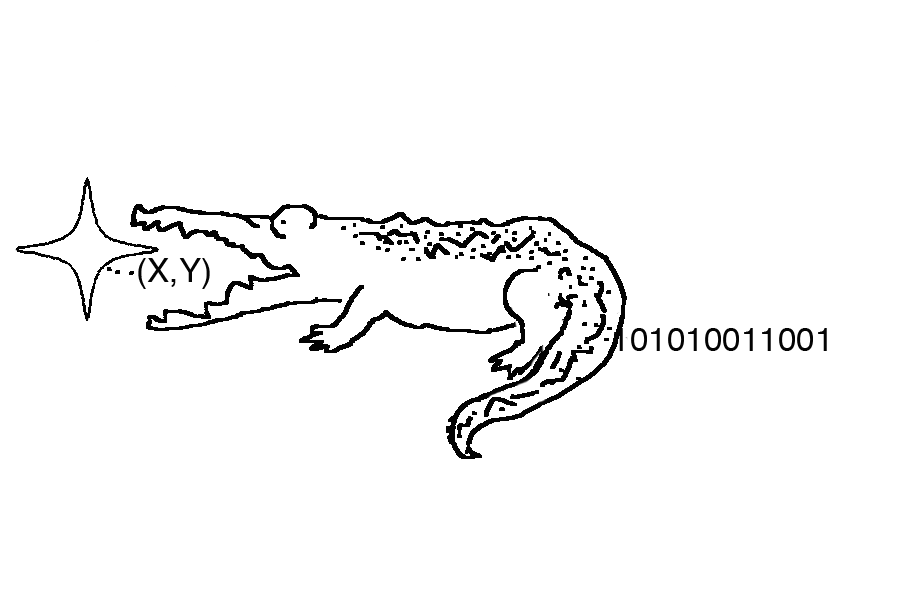
\includegraphics[width=0.45\linewidth,trim=0 35 0 40,clip]{elligator.png}
  \caption{Visualization of the Elligator encoding function $\iota^{-1}$.}
\end{figure}

In elliptic-curve cryptography, public keys and protocol messages are
elements of $E(\mathbb{F}_q)$. These objects are defined by algebraic
structure and are therefore recognizable, which can reveal the presence
of cryptographic communication.

Elligator removes this leakage by providing a formally specified interface:
\begin{itemize}
    \item Decoding function $\iota : \{0,1\}^n \rightarrow E(\mathbb{F}_q) $ unveils bitstrings to curve points
    \item Encoding function $\iota^{-1} : E(\mathbb{F}_q) \rightarrow \{0,1\}^n$ hides curve points as bitstrings
    \item Ensures efficiently computational indistinguishability from random data
\end{itemize}

\begin{table}
  \centering
  \begin{tabular}{p{0.46\linewidth} p{0.46\linewidth}}
    \toprule
    \textbf{Before} & \textbf{After} \\
    \midrule
    Paper proofs & Machine-verified proofs \\
    Finite numerical tests & Universal correctness \\
    Implementations + unit tests & Single verified specification \\
    Implicit assumptions & Explicit formalization \\
  \end{tabular}
\end{table}

\end{block}

\end{column}

\separatorcolumn

\begin{column}{\colwidth}

\begin{alertblock}{From Paper Theory to Bytecode}

\begin{center}
\begin{tikzpicture}[
    >=latex,
    node distance=1.8em,
    flow/.style={->,thick},
]

\node (papers)
{
    \includegraphics[width=.95\linewidth]{paper-stack.png}
};

\node[
    draw,
    rounded corners,
    fill=white,
    align=left,
    text width=22cm,
    inner sep=8pt,
    below=of papers
] (formal) {

{\ttfamily
import Mathlib\\
...\\
variable \{F : Type\*\} [Field F] [Fintype F]\\
variable \{q : $\mathbb{N}$\} (q\_h1 : card F = q) (q\_h2 : IsPrime q)\\
...\\
def b : $\mathbb{N}$ := Nat.log 2 q\\
def $\sigma$ ($\tau$ : Fin b $\to$ Bool) : F :=\\
\quad $\sum$ i : Fin b, if $\tau$ i then 2\^{}i else 0\\
def S : Finset ((Fin b) $\rightarrow$ Bool) :=\\
\quad filter (fun $\tau$ => ($\sigma~\tau$) $\le$ (q - 1) / 2)\\
def $\phi$ (t : F) : F $\times$ F := ...\\
def $\iota$ ($\tau$ : S) := $\phi$ ($\sigma$ $\tau$)\\
...\\
theorem S\_card : S.card = (q + 1) / 2 := by ...\\
theorem $\iota$\_injective : Injective $\iota$ := by ...\\
theorem $\iota$\_S\_eq\_$\phi$\_F : range $\iota$ = range $\phi$ := by ...\\
}
};

\node[
    draw,
    rounded corners,
    fill=white,
    align=center,
    font=\ttfamily\small,
    text width=15cm,
    inner sep=8pt,
    below=of formal
] (lambda) {
$...\left( \lambda f. \left( \lambda x. f (x x) \right) \left( \lambda x. f (x x) \right) \right)
\left( \lambda g. \lambda s. \lambda x. g s (x s f) \right)...$
};

\node[
    draw,
    rounded corners,
    fill=white,
    align=center,
    font=\ttfamily\small,
    text width=15cm,
    inner sep=8pt,
    below=of lambda
] (bytecode) {
$...10110111010101111101010000111111001101010001100...$
};


\draw[flow] (papers) -- node[midway, align=center]{
~~~~~~~~~~~~~translation into~~~formalization language
} (formal);

\draw[flow] (formal) -- node[midway, align=center]{
~~~verified by~~~Lean kernel
} (lambda);

\draw[flow] (lambda) -- node[midway, align=center]{
~~~bytecode~~~generation
} (bytecode);

\node[
    below=2em of bytecode,
    align=center
] (applications)
{

\includegraphics[width=.05\linewidth]{tor.png},

\includegraphics[width=.05\linewidth]{signal.png},

\includegraphics[width=.05\linewidth]{crypto.png}, ...
\\
{\small Tor, Signal, Bitcoin, ...}
};

\draw[flow] (bytecode.south) -- node[midway, align=center]{potentially~~~used by~~~~} (applications.north);

\end{tikzpicture}
\end{center}

\end{alertblock}

\begin{block}{Contribution}
\begin{itemize}
    \item First formalization of Elligator theory
    \item Development of specialized number theory lemmas
    \item Making implicit assumptions explicit
\end{itemize}
\end{block}

\begin{block}{Outlook}
Recent advances in \textbf{AI} have dramatically increased the amount of generated
code, documentation, and mathematical content.

This raises a fundamental question:\\
\begin{center}
\emph{How can we trust automatically generated results?}
\end{center}

Formal verification provides an objective foundation for answering this
question by reducing correctness claims to machine-checkable proofs.

Future AI systems may not only generate software and mathematical arguments,
but also the formal evidence required to verify them.

\end{block}

\begin{block}{References}
\nocite{*}
\footnotesize{\bibliographystyle{plainnat}\bibliography{poster}}
\end{block}

\end{column}

\separatorcolumn
\end{columns}
\end{frame}

\end{document}
